\section{数据分析}
距离是评价机器鼠行为交互的重要指标之一,图\ref{figure_distance}为图\ref{figure_heatmap}中各阶段$1~min$内距离变化情况。该图显示,在训练初期,二者距离变化较少,这与图\ref{figure_heatmap}\subref{figure_heatmap_start}中存在的两处学习鼠停留较长位置相符。
\begin{figure}[htb]
  %\vspace{13pt}
  \centering
  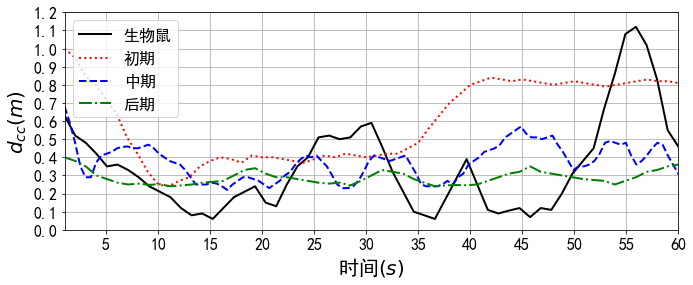
\includegraphics[height=5cm]{images/ch05/distance.png}
  \caption{机器鼠间的距离变化($1~min$)}\label{figure_distance}
\end{figure}

在进入训练中期后,学习鼠能够更频繁地进入与规则鼠开展有效交互地距离($d_{cc}<0.3~m$)范围($13\sim22~s$,$35\sim39~s$和$27\sim29~s$等),这表明了学习鼠已经学习到部分有利于行为交互的规则。

在训练后期,学习鼠能够频繁进入规则鼠的有效交互距离以内,同时,当两者距离超出这一范围时,由于学习鼠经训练获得的跟随特性,其能够迅速重新建立行为交互的联系。但与生物鼠相比,机器鼠的距离变化跟平缓,且运动范围明显更小:生物鼠之间的距离最远超过$1~m$,最近距离仅为$0.06~m$,机器鼠距离始终在$0.25\sim 0.4~m$之间,这表明机器鼠的活跃程度与生物鼠存在差异。造成这种差异的原因是由于Q-学习目标的单一性(本文设定学习鼠训练目标为与规则鼠开展有效交互),学习鼠必须时刻靠近规则鼠。同时由于状态划分以$d_{cc}=0.3~m$为界限,使得学习鼠在进入这一范围后不再靠近规则鼠。

% 距离的变化情况进一步印证了学习鼠具备的跟随能力,当二者距离较近时,行为交互的合理性将依照各自的动作判定。图\ref{figure_actionseq}为训练后期仿真环境中每秒学习鼠与规则鼠的动作序列,图中色条为对此刻二者动作与Q-学习所设定的最终状态间相似性评价,评价标准为:
% \begin{enumerate}[leftmargin=0em, listparindent=2em, parsep=0em, topsep=0em, label=(\theenumi)]
% %\setlength{\leftmargin}{0em}
% \setlength{\itemindent}{4em}
% \setlength{\labelsep}{0em}
% \setlength{\labelwidth}{2em}
% \setlength{\parsep}{0em}
% \setlength{\itemsep}{0em}
% \setlength{\topsep}{0em}
% %\setlength{\listparindent}{2em}
%   \item \label{std_highest}当学习鼠与规则鼠距离较近($d_{cc}<0.3~m$),并且二者动作分别为梳理和被梳理,即此时行为表现为一方梳理另一方,达到最终状态$s_5$和$s_6$,评价最高(7)。当动作分别为攀爬和匍匐时,即表现征服和服从的行为,评价次高(6)。这些动作如图\ref{figure_stdhighest}所示。
% \begin{figure}[htb]
%   %\vspace{13pt}
%   \centering
%   \subfigure[学习鼠被梳理]{\label{figure_stdallow}
%   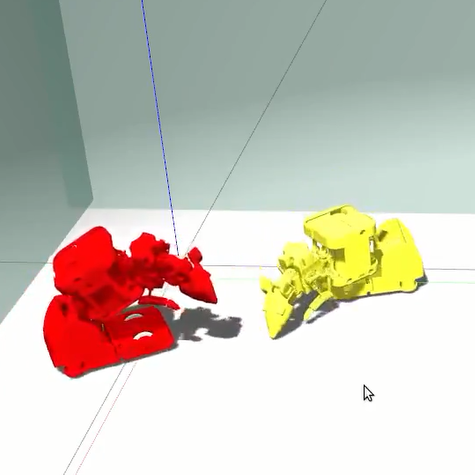
\includegraphics[width=3.5cm]{images/ch05/mature/allow.png}
%   }
%   \subfigure[学习鼠梳理规则鼠]{\label{figure_stdgroom}
%   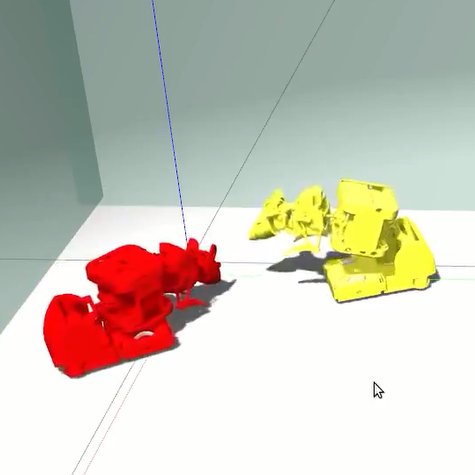
\includegraphics[width=3.5cm]{images/ch05/mature/groom.png}
%   }
%   \subfigure[学习鼠被征服]{\label{figure_stdunder}
%   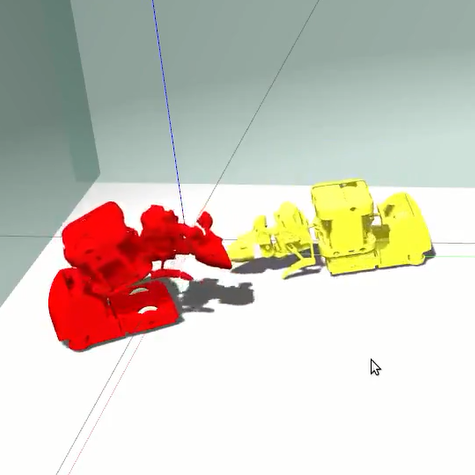
\includegraphics[width=3.5cm]{images/ch05/mature/under.png}
%   }
%   \subfigure[学习鼠征服规则鼠]{\label{figure_stdup}
%   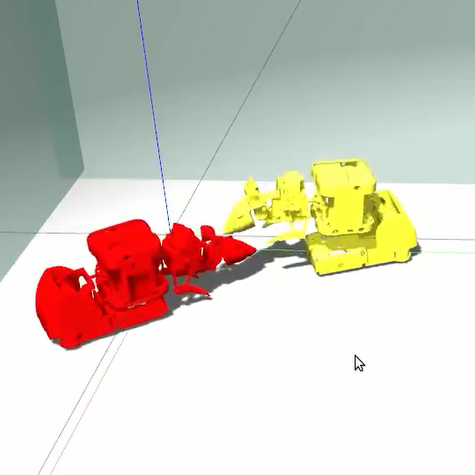
\includegraphics[width=3.5cm]{images/ch05/mature/up.png}
%   }
%   \caption{评价较高的行为}\label{figure_stdhighest}
% \end{figure}
%   \item 在不满足\ref{std_highest}的情况下,当二者距离在减小,即一方靠近另一方时,评价在2$\sim$5之间。
%   \item 当二者动作产生冲突(例如同时希望攀爬至对方身体之上),评价为0或1。
% \end{enumerate}
% \begin{figure}[htb]
%   %\vspace{13pt}
%   \centering
%   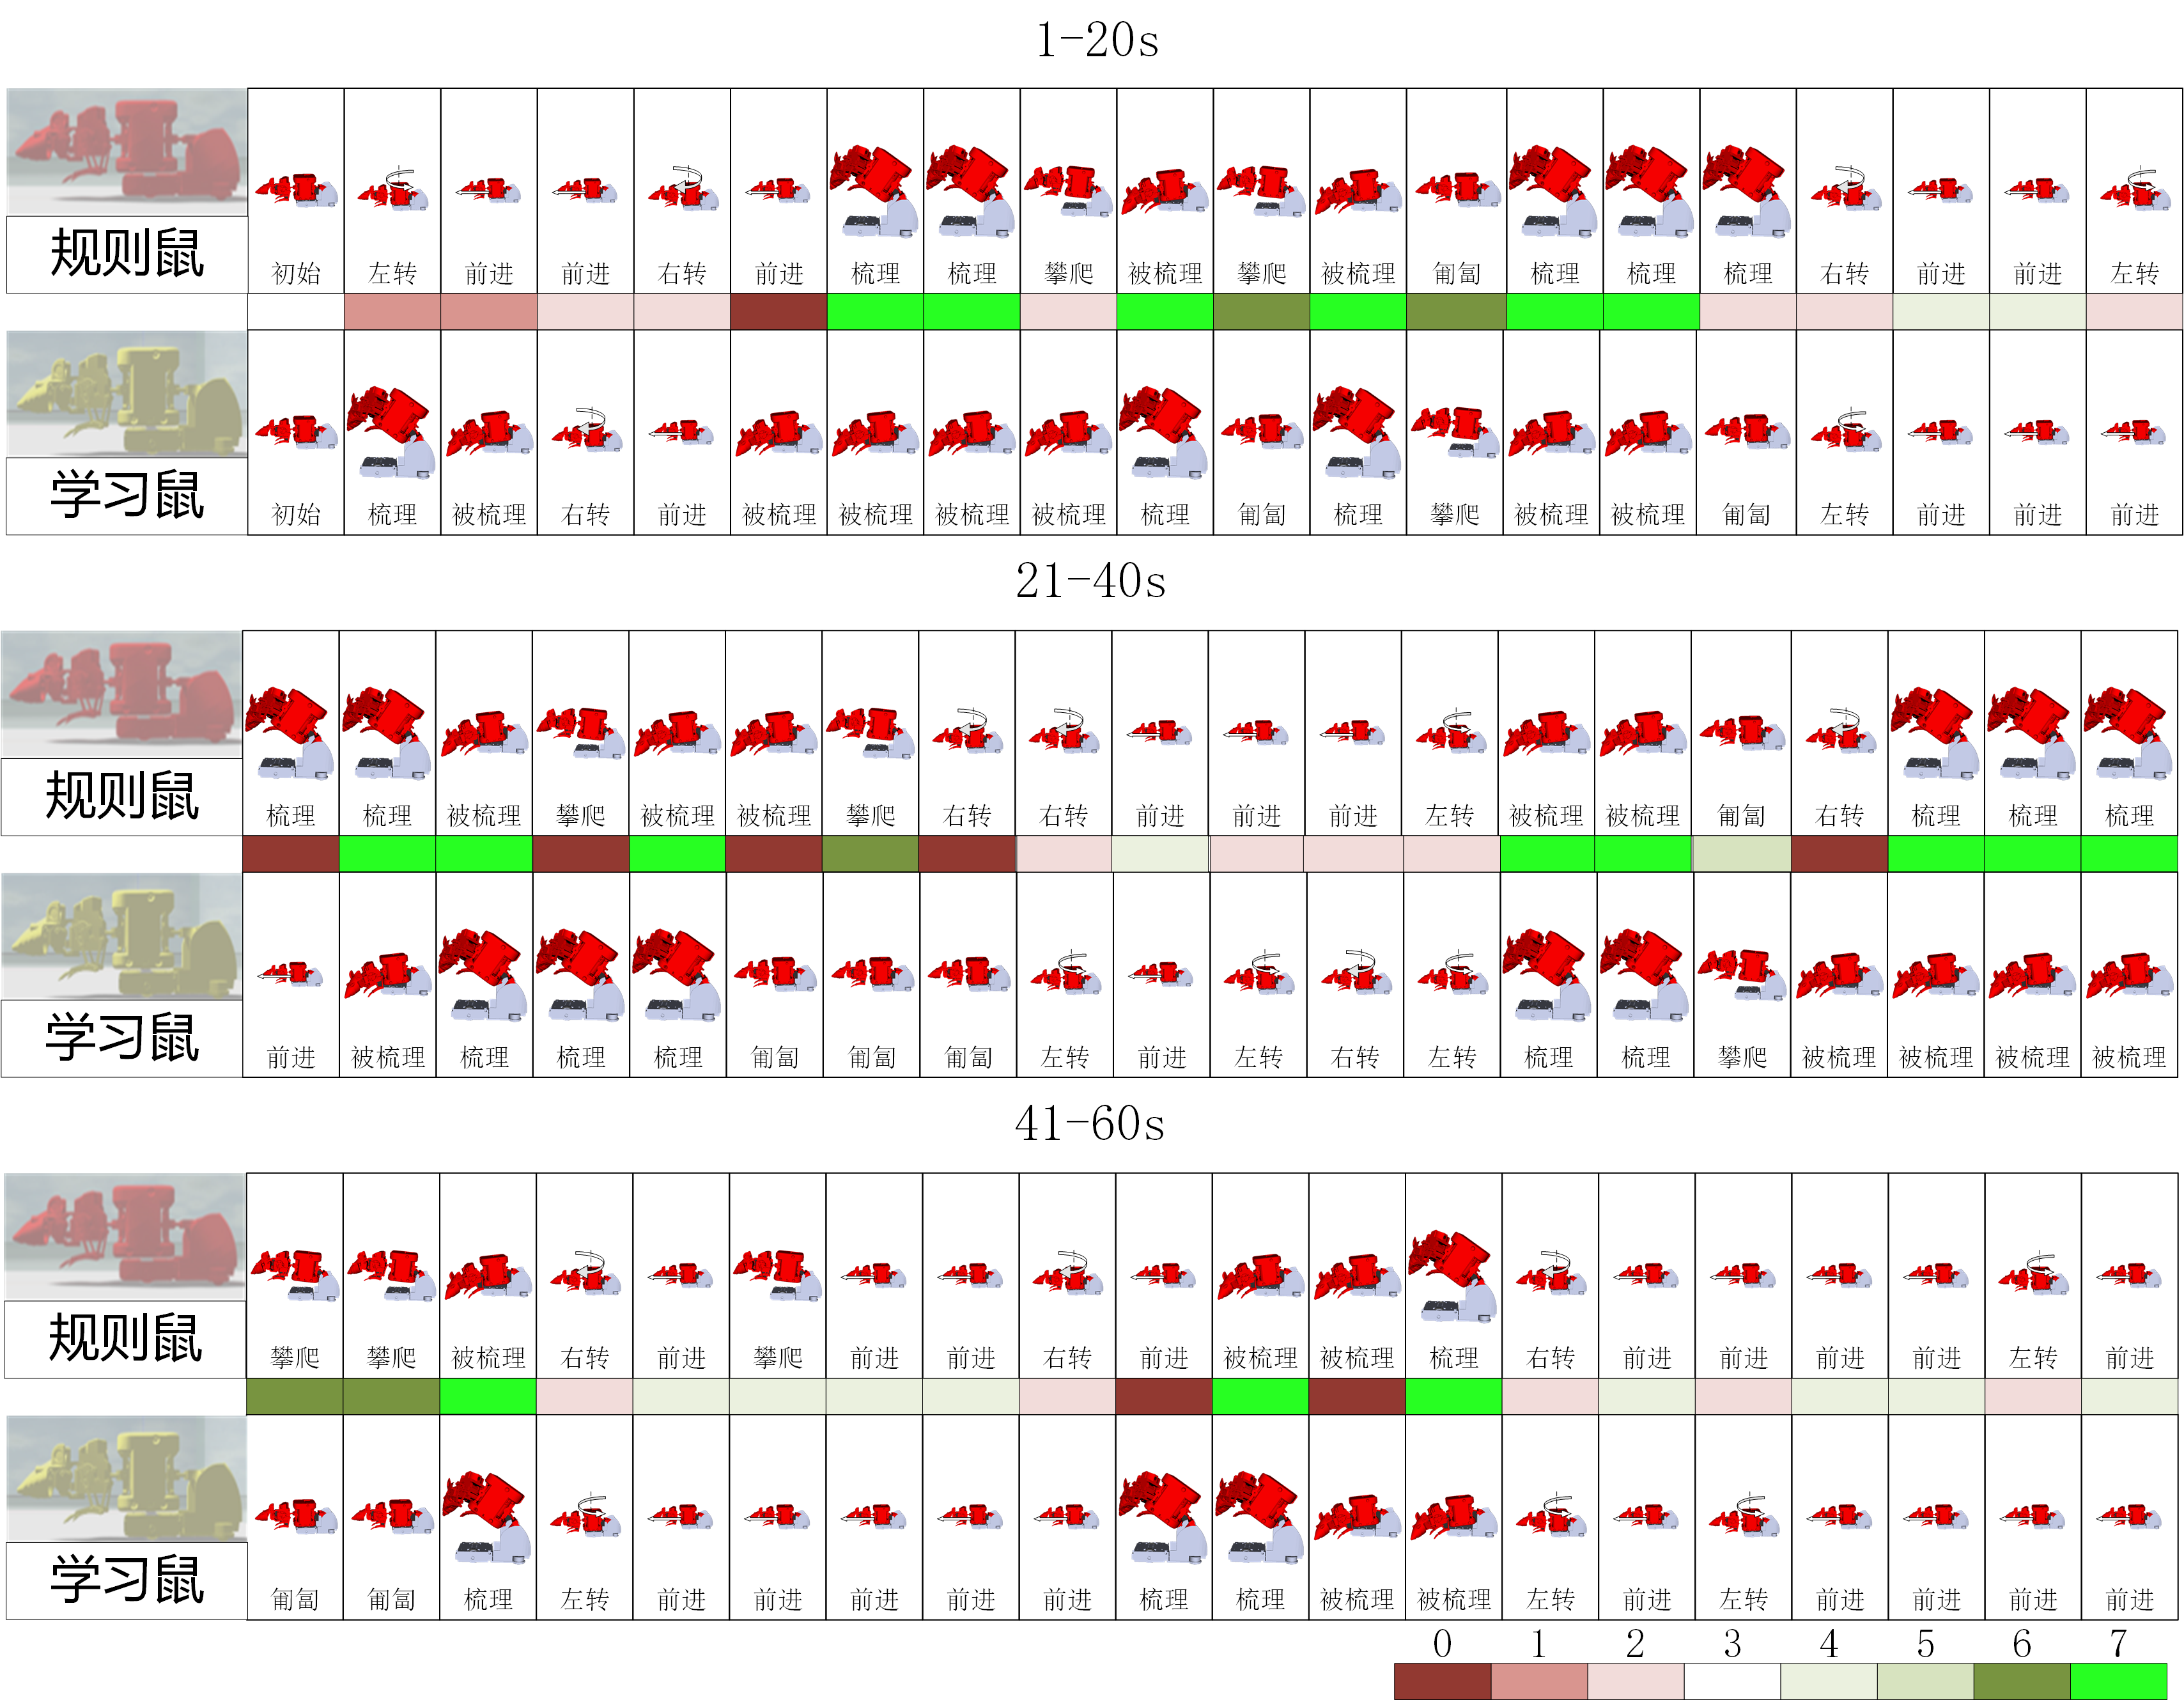
\includegraphics[width=1\linewidth]{images/ch05/mature/actionseq.png}
%   \caption{机器鼠动作序列($1~min$)}\label{figure_actionseq}
% \end{figure}

% 图\ref{figure_actionseq}显示,尽管在仿真中机器鼠出现表现不协调的时刻(评价为0),但这些时刻出现的频率较低(约为$13\%$),并且能够被迅速纠正(图中评价为0的时刻之后往往评分最高)。而具有较高相似度的动作持续时间一般较长,不易终止。表明这一阶段的学习鼠能够及时根据规则鼠的动作调整自身的动作,并且能以合适的方式引发规则鼠的交互行为。

% 表\ref{tab:action_con}展示了这$1~min$内各种行为的表现时间,通过对比生物鼠与仿生机器鼠各种行为表现时间发现,二者各种行
% \begin{table}[htbp]
%   \linespread{1.5}
%   \zihao{5}
%   \centering
%   \caption{训练后期$1~min$内行为模式时间统计$(s)$}\label{tab:action_con}
%   \begin{tabular}{*{1}{>{\centering\arraybackslash}m{1.5cm}}m{2.5cm}<{\centering\arraybackslash}*{2}{>{\centering\arraybackslash}m{0.8cm}}m{2.5cm}<{\centering\arraybackslash}*{2}{>{\centering\arraybackslash}m{0.8cm}}}
%     \toprule
%     行为 & 征服与服从 & 梳理 & 嗅探 & 跟随/接近 & 远离 & 其他 \\ \midrule
%     机器鼠 & 5 & 17 & 8 & 21 & 3 & 6 \\
%     生物鼠 & 8 & 13 & 9 & 17 & 6 & 7 \\
%     \bottomrule
%     \end{tabular}
% \end{table}
% 为的持续时间具有相似性,但生物鼠能够表现仿生机器鼠难以表达的不交互的特征。这与强化学习的原理相关,在以有效行为交互为目标的情况下,学习鼠会尽可能避免一些非交互行为,而这一点也值得改进。同时,在征服与服从、梳理、嗅探这三种典型的两只生物鼠交互行为的时间比较上,机器鼠与生物鼠表达一致。

上述分析表明了基于强化学习的仿生机器鼠行为交互具有良好的适应规则鼠随机性的能力,仿生机器鼠能够在仿真平台中表达与生物鼠相似的行为交互。